\documentclass{tufte-handout}

\title{Funkcijų transformacijos}

\author[Vilius Paliokas]{Vilius Paliokas}

\date{2023-02-01} % without \date command, current date is supplied

%\geometry{showframe} % display margins for debugging page layout

\usepackage[main=lithuanian]{babel}
\usepackage[utf8]{inputenc}

\usepackage{tikz}
\usepackage{tikz-cd}
\usepackage{pgfplots}

\usepackage{booktabs}
\usepackage{isotope}
\usepackage{siunitx}
\sisetup{
  per-mode = fraction,
  load-configurations = abbreviations,
}

\usepackage{graphicx} % allow embedded images
\setkeys{Gin}{width=\linewidth,totalheight=\textheight,keepaspectratio}
\graphicspath{{graphics/}} % set of paths to search for images
\usepackage{amsmath}  % extended mathematics
\usepackage{booktabs} % book-quality tables
\usepackage{units}    % non-stacked fractions and better unit spacing
\usepackage{multicol} % multiple column layout facilities
\usepackage{lipsum}   % filler text
\usepackage{fancyvrb} % extended verbatim environments
\fvset{fontsize=\normalsize}% default font size for fancy-verbatim environments

% Standardize command font styles and environments
\newcommand{\doccmd}[1]{\texttt{\textbackslash#1}}% command name -- adds backslash automatically
\newcommand{\docopt}[1]{\ensuremath{\langle}\textrm{\textit{#1}}\ensuremath{\rangle}}% optional command argument
\newcommand{\docarg}[1]{\textrm{\textit{#1}}}% (required) command argument
\newcommand{\docenv}[1]{\textsf{#1}}% environment name
\newcommand{\docpkg}[1]{\texttt{#1}}% package name
\newcommand{\doccls}[1]{\texttt{#1}}% document class name
\newcommand{\docclsopt}[1]{\texttt{#1}}% document class option name
\newenvironment{docspec}{\begin{quote}\noindent}{\end{quote}}% command specification environment

\begin{document}

\maketitle% this prints the handout title, author, and date

\begin{abstract}
  \noindent
  Šioje mokomojoje medžiagoje funkcijų transformacijų teoriją ir pavyzdžius.
  Pagal bendrojo ugdymo 11 klasės matematikos bendrojo kurso programą mokiniai
  turi mokėti, kaip atliekamos $y=f(x)+a$, $y=f(x+a)$, $y=-f(x)$, $y=a\cdot
    f(x)$
  formulėmis aprašomos transformacijos. Čia taip pat pateikiamos šių
  transformacijų pasireiškimai įvairaus konteksto situacijose. Funkcijų
  transformacijoms suprasti, pirmiausia plėtojama samprata apie funkcijas ir jų
  savybes.
\end{abstract}

% \printclassoptions
\section{Funkcijos samprata}\label{se c:page-layout}

Dažnu atveju, funkcija yra asocijuojama su $f(x)$ žymėjimu, o šį mes skaitome
\textit{ef nuo iks}. Po $f(x)$ visada seka kažkoks tai
reiškinys, dažniausiai tai būna tiesinis reiškinys $ax+b$ (pvz.:
$f(x)=x+1$) ar
kvadratinis reiškinys $ax^2+bx+c$ (pvz.: $f(x)=x^2$). O vėliau, mokyklos kurse
sutiksime ir kitokio
tipo funkcijas.

Toliau prisiminsime apie aibes ir pamatysime, kaip jos susijusios su
funkcijomis.

\subsection{Apie aibes}\label{sec:about_sets}

Kadangi jau susipažinome su aibėmis, galime pasigilinti, kaip aibės
susijusios su funkcijomis. Bet pirma prisiminsime keletą aibių
teorijos\footnote{Aibių teorija yra matematikos šaka, kurioje nagrinėjamos
  aibės - objektų rinkiniai} aspektų. \textbf{Aibė} - rinkinys	objektų, kurie
vadinasi aibės elementais. Aibės elementu gali būti bet kas (obuoliai,
planetos, mašinos), o jie yra susieti viena (ar daugiau) bendra
savybę. Matematikoje nagrinėjami matematiniai objektai, mokyklos matematikos
programoje nagrinėjamos
tik skaičių aibės. Jeigu elementas $x$ priklauso aibei $X$, tai užrašoma $x \in
  X$. Jeigu elementas $x$ nepriklauso aibei $X$, tai rašome $x \notin X$.

Priklausomai nuo elementų skaičiaus aibėje, aibės gali būti baigtinės arba
begalinės. Baigtinės aibės atveju mes galime suskaičiuoti šios elementus, juos
nesunkiai visus išvardinti. Pavyzdžiui turime aibę
$$A=\{0; 1; 4; 9; 16; 25\} $$
Ši aibė turi baigtinį kiekį elementų - ją sudaro 6 elementai. Natūraliųjų
skaičių aibė $\mathbb{N}$ yra vienas iš begalinės aibės pavyzdžių, ši aibė turi
be galo daug
elementų ($1;2;3;4;5;6;7;8\ldots$).

\subsection{Aibės ir funkcijos}\label{sec:about_sets_and_functions}

O dabar bandysime atsakyti į klausimą, kaip susijusios aibės ir funkcija.
Tarkime turime dvi aibes $X$ ir $Y$ (paskui bus ir konkretūs pavyzdžiai).
Paprastumo dėlei, šios aibės bus baigtinės abi sudarytos iš keturių elementų:

$$X = \{x_{1},x_{2},x_{3},x_{4}\};$$
$$Y = \{y_{1},y_{2},y_{3},y_{4}\};$$

Šių grafinis atvaizdavimas pažymėtas žemiau,
\ref{fig:function_as_sets_elements_relation} paveiksle. Kol kas pavaizduotas
rodykles ignoruokime.

\begin{figure}[!htpb]
  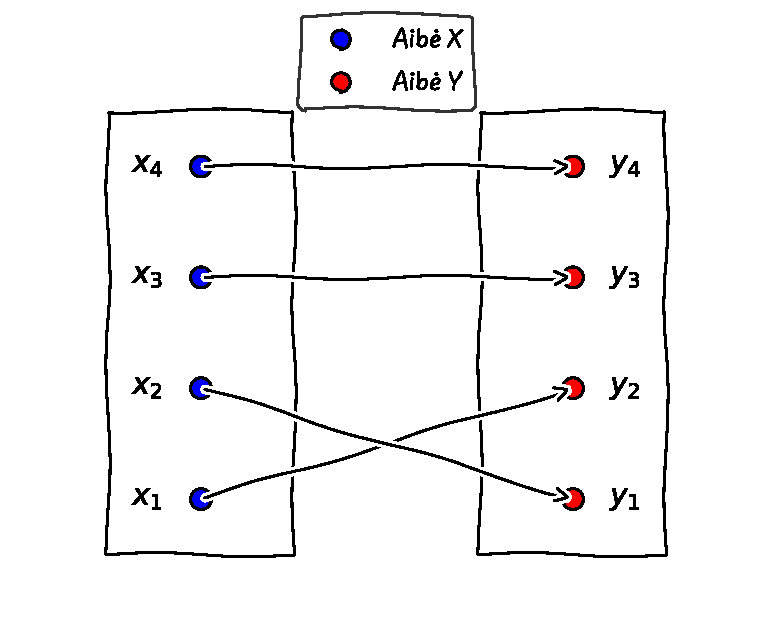
\includegraphics{./graphs/functions_as_graphs.pdf}
  \caption{Funkcija, kaip aibių elementų sąryšiai}
  \label{fig:function_as_sets_elements_relation}
  \setfloatalignment{c}
\end{figure}

O dabar svarbiausia dalis. Kiekvienam aibės $X$ elementui priskyrus elementą iš
aibės $Y$ gauname tam tikrus ryšius tarp šių dviejų aibių. Tarkime, anksčiau
paminėtiems elementams iš aibės $X$ priskirkime elementą iš aibės $Y$:
\begin{itemize}
  \item $x_1 \rightarrow y_2$;
  \item $x_2 \rightarrow y_1$;
  \item $x_3 \rightarrow y_3$;
  \item $x_4 \rightarrow y_4$;
\end{itemize}

Šiuos ryšius tarp dviejų aibių elementų galime matyti
\ref{fig:function_as_sets_elements_relation} paveiksle, jie pavaizduoti
rodyklėmis. Rodyklė $\rightarrow$ yra priskirimo veiksmas matematikoje. Jeigu
visų aibės $X$ elementų priskyrimo aibės $Y$ elementams veiksmą pavadintume
$f$, tai galėtume
pažymėti:
$$ f: X \rightarrow Y  \quad\text{arba}\quad  X \xrightarrow{f} Y$$

Iki šio momento turėjote pamatyti pažįstamų dalykų: $f$, $x$, $y$. Jei
kiekvienas aibės $X$ elementas yra susijęs su vienu ir tik vienu kitos aibės
$Y$ elementu, tai toks priskyrimas (ryšys) vadinamas
\textbf{funkcija}\footnote{Labai
  svarbi šio apibrėžimo dalis yra ta, kad vienas (ir tik vienas) elementas
  priskiriamas kitam aibės elementui, kitu atveju tai negali vadintis
  funkcija}. O tai užrašoma $y=f(x)$.

\subsection{Funkcijos sąvokos}\label{sec:function_related_defintions}

Kalbant apie funkcijas, būtina žinoti su funkcija susijusiąs sąvokas. Šios
sąvokos ateina iš funkcijos apibrėžimo:

\begin{itemize}
  \item $x$ - funkcijos nepriklausomas kintamasis arba funkcijos argumentas;
  \item $y$ - funkcijos priklausomas kintamasis arba funkcijos reikšmė;
  \item $X$ - visos galimos $x$ reikšmės arba funkcijos $f(x)$ apibrėžimo
        sritis. Ši sritis dažnai žymima $D(f)$;
  \item $Y$ - visos galimos $y$ reikšmės arba funkcijos $f(x)$ reikšmių sritis.
        Ši sritis dažnai žymima $E(f)$;
  \item $f$ - taisykė, pagal kurią $x$ reikšmėms priskiriamos $y$ reikšmės;
\end{itemize}

Šių sąvokų atikmenis galima pamatyti anksčiau pavaizduotame
\ref{fig:function_as_sets_elements_relation} paveiksle. Pavyzdžiui, paveiksle
mėlyni rutuliukai $x_1, x_2, x_3, x_4$ yra funkcijų argumentai, o jų visuma
(apibrėžta sritis) yra apibrėžimo sritis. Reikšmių sritis yra apibrėžta sritis
su raudonai $y_1, y_2, y_3, y_4$ taškais. Visų rodyklių visuma yra taisyklė
$f$, pagal kurią vieni aibės (apibrėžimo srities) elementai priskiriami kitiems
aibės (reikšmių srities) elementams.

\subsection{Funkcijos pavyzdys}\label{sec:function_example}

Turime dvi aibes:
$$X =\{0; 1; 2; 3; 4; 5\}$$
$$Y =\{0; 1; 4; 9; 16; 25\}$$

Dabar priskirkime aibės $X$ vienam ir tik vienam kitos aibės $Y$ elementą:
\begin{itemize}
  \item $0 \rightarrow 0$;
  \item $1 \rightarrow 1$;
  \item $2 \rightarrow 4$;
  \item $3 \rightarrow 9$;
  \item $4 \rightarrow 16$;
  \item $5 \rightarrow 25$;
\end{itemize}

Šį priskyrimą pavadinkime $f$. Dabar, šių skaičių ryšį galima parašyti $y=f(x)$
arba $f(x)=y$  forma:
\begin{itemize}
  \item $f(0) = 0$;
  \item $f(1) = 1$;
  \item $f(2) = 4$;
  \item $f(3) = 9$;
  \item $f(4)= 16$;
  \item $f(5) = 25$;
\end{itemize}

Šiuos ryšius galima pavaizduoti ir grafiškai:

\begin{figure}[!htpb]
  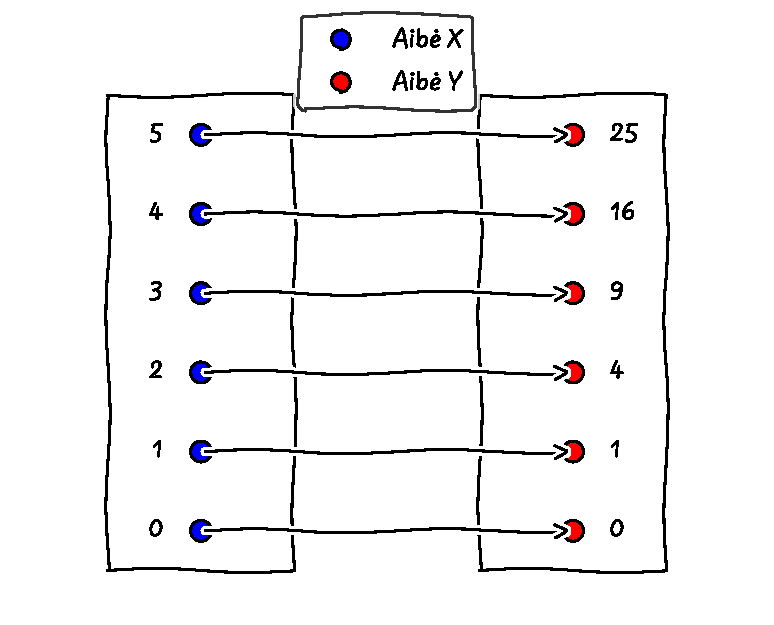
\includegraphics{./graphs/functions_as_graphs_example1.pdf}
  \caption{Aibės $X =\{0; 1; 2; 3; 4; 5\}$ elementų priskyrimas aibės $Y =\{0;
      1; 4; 9; 16; 25\}$ elementams}
  \label{fig:function_as_set_example}
  \setfloatalignment{c}
\end{figure}

Šią funkcinę priklausomybę galima ir apibūdinti:
\begin{itemize}
  \item Funkcijos apibrėžimo sritis yra $\{0; 1; 2; 3; 4; 5\}$;
  \item Funkcijos reikšmių sritis yra $\{0; 1; 4; 9; 16; 25\}$;
  \item Mažiausia reikšmė ($y$) yra 0, kai argumentas ($x$) yra lygus 0;
  \item Didžiausia reikšmė ($y$) yra 25, kai argumentas ($x$) yra lygus 5;
\end{itemize}

\subsection{Funkcijos reiškinys}\label{sec:function_example}

Funkciją galima aprašyti reiškiniu. Ta daroma, nes neįmanoma išrašyti visų
begalinių ryšių tarp dviejų begalinių aibių. Šiuos reiškinius jau analizavote
ir ankstesnėse klasėse. Anksčiau pateiktame pavyzdyje, galima įžvelgti tam
tikrą dėsningumą. Funkcijos reikšmės buvo gautos argumentus pakėlus kvadratu.
Tokią bendrą taisyklę visiems skaičiams ($x\in \mathbb{R}$) galima užrašyti
taip:
$$f(x)=x^2$$

\begin{marginfigure}%

  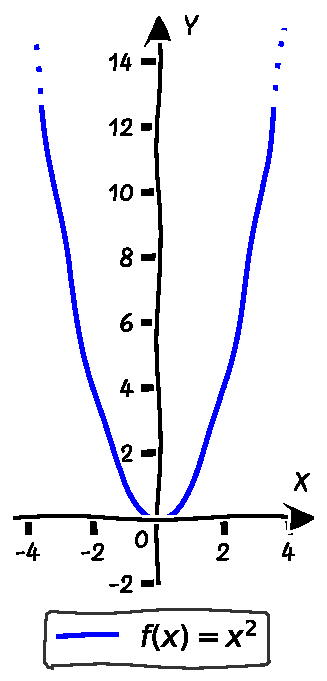
\includegraphics[width=\linewidth]{./graphs/quadratic_function_plot_example.pdf}
  \caption{$f(x)=x^2$ grafikas $OXY$ koordinačių plokštumoje}
  \label{fig:example_quadratic_plot}
\end{marginfigure}

Tai reiškia, kad kiekviena funkcijos reikšmė gaunama argumentą, iš apibrėžimo
srities, pakėlus kvadratu. Tokiu būdu gaunama begalė argumentų $x$ ir reikšmių
$y$ skaičių porų
$(x; y)$. Šiuos taškus atvaizdavus koordinačių plokštumoje $OXY$ gaunamas
funkcijos grafikas (\hyperref[fig:example_quadratic_plot]{paveikslas
  \ref*{fig:example_quadratic_plot}}).

\section{Grafikų transformacija}\label{sec:graph_transformation}

Tarkime turime žinome, kaip atrodo funkcijos grafikas, jį modifikuojame taip,
kad sukurtume panašus, bet kitoks to grafikos variantas. Toks procesas
vadinamas funkcijos grafiko transformacija. Matematikos bendrajame kurse reikia
žinoti 4 tipų transformacijas. Šių transformacijų pavyzdžiai matomi žemiau:

\begin{figure*}[h]
  \begin{minipage}{0.22\textwidth}
    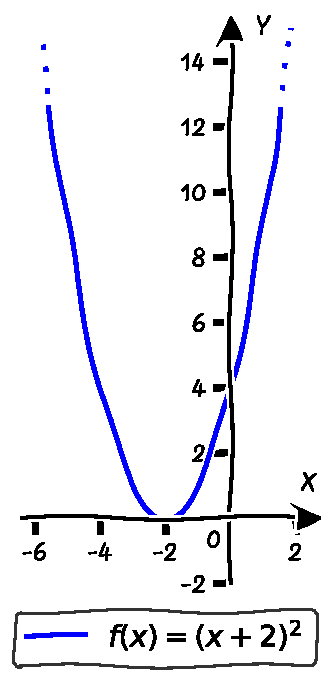
\includegraphics[width=\linewidth]{./graphs/quadratic_func_lsh_2.pdf}
    \label{fig:first}
  \end{minipage}\hfill
  \begin{minipage}{0.30\textwidth}
    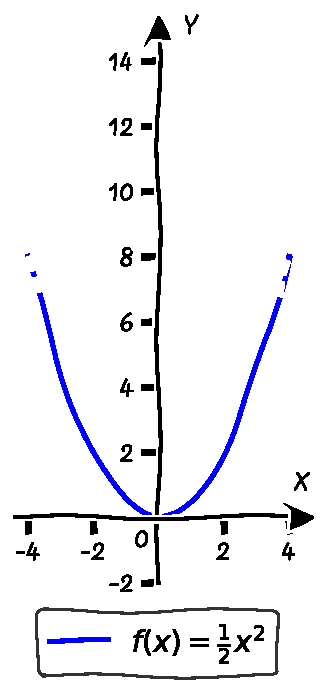
\includegraphics[width=\linewidth]{./graphs/quadratic_func_shrink_2.pdf}
    \label{fig:second}
  \end{minipage}\hfill
  \begin{minipage}{0.21\textwidth}
    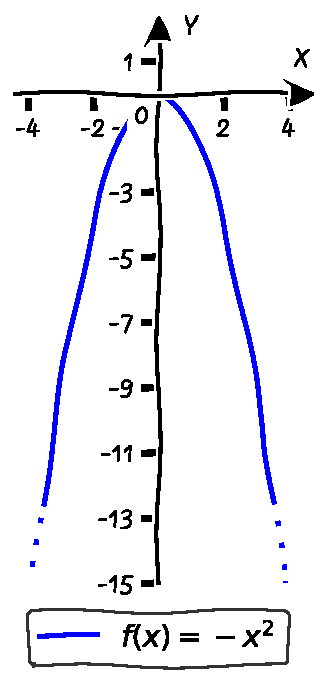
\includegraphics[width=\linewidth]{./graphs/quadratic_func_flipped.pdf}
    \label{fig:third}
  \end{minipage}\hfill
  \begin{minipage}{0.21\textwidth}
    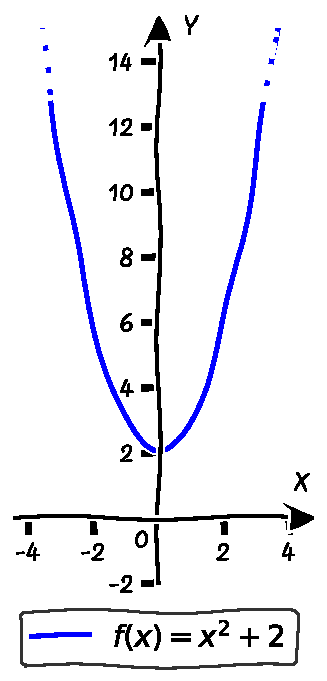
\includegraphics[width=\linewidth]{./graphs/quadratic_func_ush_2.pdf}
    \label{fig:fourth}
  \end{minipage}
  \caption{$f(x)=x^2$ grafiko transformacijos: $y=f(x-2)$, $y=\frac{1}{2}f(x)$,
    $y=2f(x)$, $y=f(x)+2$ }
\end{figure*}

Šie visi grafikai atrodo panašiai, bet skiriasi nuo pradinės funkcijos
$f(x)=x^2$ grafiko, nes atlitkos tam tikros transformacijos:

\begin{itemize}
  \item Postūmis OX ašimi $y=f(x+a)$, čia $a \in \mathbb{R}$;
  \item Postūmis OY ašimi $y=f(x)+b$, čia $b \in \mathbb{R}$;
  \item Ištempimas, sutraukimas $y=c \cdot\ f(x)$, čia $c \in \mathbb{R}$;
  \item Apvertimas OX ašies atžvilgiu $y=-f(x)$;
\end{itemize}

Toliau giliau analizuosime šių transformacijų poveikį grafikams, jų taškams.
Įsivaizduokime turime funkcijos $f(x)$ tašką $(a, b)$, tai tokiu atveju $f(a) =
  b$. \hyperref[tbl:after_transformations]{\ref*{tbl:after_transformations}
  lentelėje
} pavaizduota, kaip keičiasi funkcijos taškai $(a, b)$ ir grafikas,
modifikuojant
funkcijos $f(x)$ reikšmę.

\begin{table*}[!htpb]
  \centering
  \begin{tabular}{
      S |
      S[separate-uncertainty = true] |
      S[table-format = 5]
    }
    \toprule
    Transformacija                    & {Kaip pasikeičia $f(x)$ grafiko
        taškai}
                                      & {Grafiko vizualinis pokytis}        \\
    \midrule
    {$f(x)+d$, $d>0$}                 & {$(a,b)\mapsto(a, b+d)$}
                                      & {Kyla viršun per $d$}               \\
    {$f(x)-d$, $d>0$}                 & {$(a,b)\mapsto(a, b-d)$}
                                      & {Leidžiasi žemyn per $d$}           \\
    {$c \cdot f(x)$, $c>0$}           & {$(a,b)\mapsto(a, c \cdot b)$}
                                      & {Išsitempia vertikaliai per $c$}    \\
    {$\frac{1}{c} \cdot f(x)$, $c>0$} & {$(a,b)\mapsto(a, \frac{1}{c} \cdot
          b)$}
                                      & {Susitraukia vertikaliai per $c$}   \\
    {$-f(x)$}                         & {$(a,b)\mapsto(a, -b)$}
                                      & {Apsiverčia $OX$ ašies atžvilgiu}   \\
    \bottomrule
  \end{tabular}
  \vspace{16pt} % Adjust the space as needed
  \caption{Funkcijų transformacijos, modifikuojant jos reikšmę}.
  \label{tbl:after_transformations}
\end{table*}

\subsection{Pavyzdys}\label{sec:function_transformation_example}

Pavaizduosime konkrečius pavyzdžius
aprašytoms transformacijoms
\hyperref[tbl:after_transformations]{\ref*{tbl:after_transformations}
  lentelėje}. Tam naudosime jau anksčiau naudotą $f(x)=x^2$ funkciją.
Pažiūrėsime, koks pokytis, kai nubrėžus $f(x)+2$,  $f(x)-2$,
$2f(x)$,$\frac{1}{2}f(x)$,$-f(x)$. Šituos brėžinius rasite
\hyperref[sec:function_transformation_example]{\pageref*{fig:function_transformation_example}
  puslapyje}
  
\begin{figure*}[p]
  \begin{fullwidth}
    \centering
    % First row
    \hspace*{-205pt} % Adjust this value as needed
    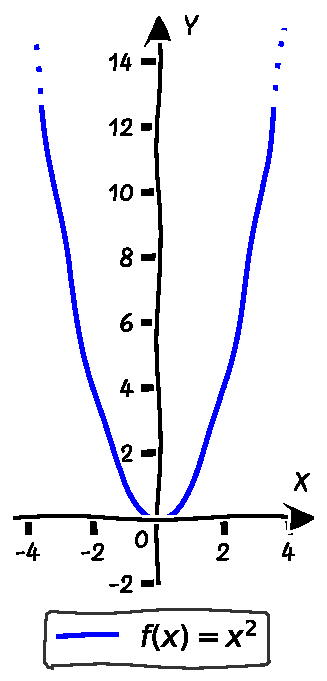
\includegraphics[width=0.32\linewidth]{./graphs/quadratic_func_primary.pdf}\hspace{5pt}
    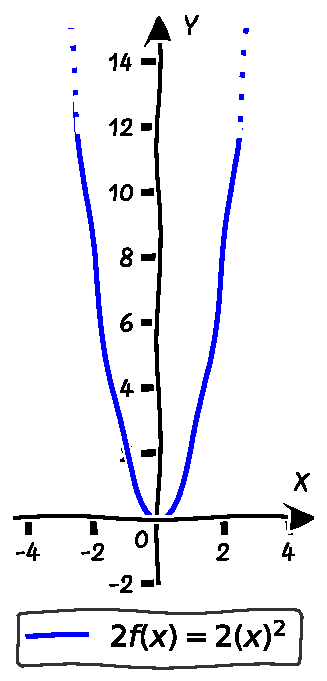
\includegraphics[width=0.25\linewidth]{./graphs/quadratic_func_transform_2.pdf}\hspace{5pt}
    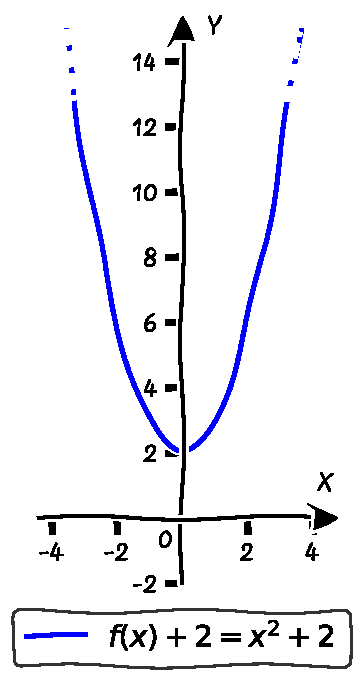
\includegraphics[width=0.32\linewidth]{./graphs/quadratic_func_transform_3.pdf}
    \\\vspace{\baselineskip}

    % Second row
    \hspace*{-205pt} % Keep this value consistent with the first row
    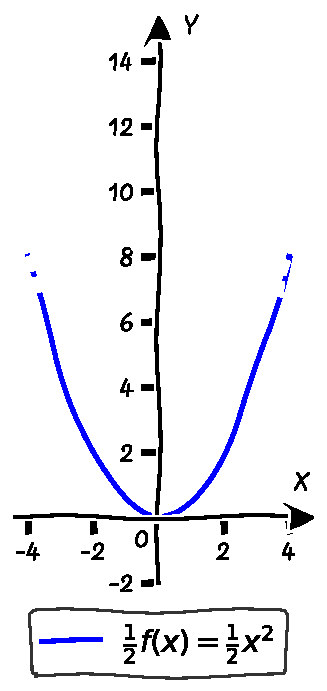
\includegraphics[width=0.3\linewidth]{./graphs/quadratic_func_transform_4.pdf}\hspace{5pt}
    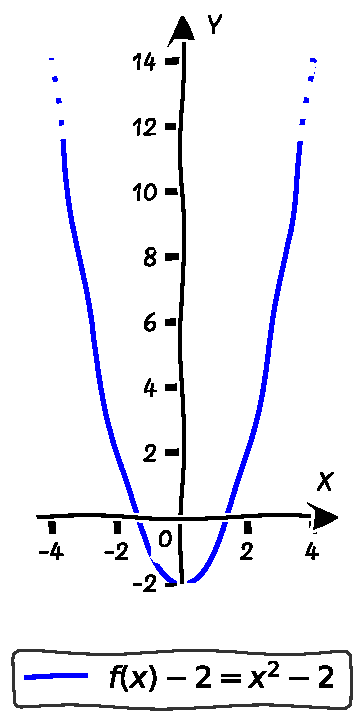
\includegraphics[width=0.3\linewidth]{./graphs/quadratic_func_transform_5.pdf}\hspace{5pt}
    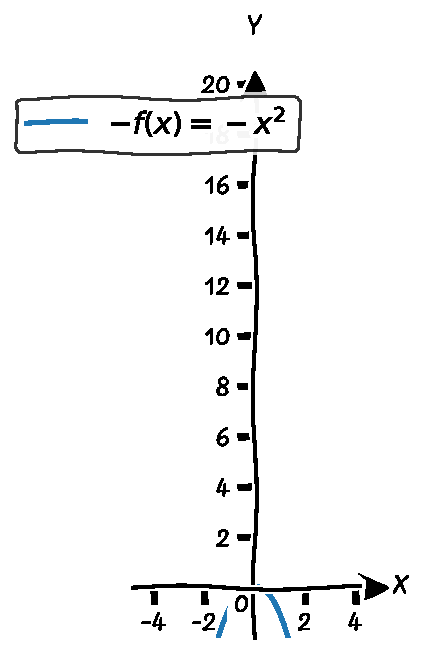
\includegraphics[width=0.3\linewidth]{./graphs/quadratic_func_transform_6.pdf}
  \end{fullwidth}
  \label{fig:function_transformation_example}
\end{figure*}

\section{Page Layout}\label{sec:page-layout}
\subsection{Headings}\label{sec:headings}
This style provides \textsc{a}- and \textsc{b}-heads (that is,
\Verb|\section| and \Verb|\subsection|), demonstrated above.

The Tufte-\LaTeX\ classes will emit an error if you try to use
\linebreak\Verb|\subsubsection| and smaller headings.

% let's start a new thought -- a new section
\newthought{In his later books},\cite{Tufte2006} Tufte
starts each section with a bit of vertical space, a non-indented paragraph,
and sets the first few words of the sentence in \textsc{small caps}.  To
accomplish this using this style, use the \Verb|\newthought| command:
\begin{docspec}
  \doccmd{newthought\{In his later books\}, Tufte starts\ldots}
\end{docspec}

\subsection{Sidenotes}\label{sec:sidenotes}
One of the most prominent and distinctive features of this style is the
extensive use of sidenotes.  There is a wide margin to provide ample room
for sidenotes and small figures.  Any \Verb|\footnote|s will automatically
be converted to sidenotes.\footnote{This is a sidenote that was entered
  using the \texttt{\textbackslash footnote} command.}	If you'd like to place
ancillary
information in the margin without the sidenote mark (the superscript
number), you can use the \Verb|\marginnote| command.\marginnote{This is a
  margin note.	Notice that there isn't a number preceding the note, and
  there is no number in the main text where this note was written.}

The specification of the \Verb|\sidenote| command is:
\begin{docspec}
  \doccmd{sidenote[\docopt{number}][\docopt{offset}]\{\docarg{Sidenote
      text.}\}}
\end{docspec}

Both the \docopt{number} and \docopt{offset} arguments are optional.  If you
provide a \docopt{number} argument, then that number will be used as the
sidenote number.  It will change of the number of the current sidenote only and
will not affect the numbering sequence of subsequent sidenotes.

Sometimes a sidenote may run over the top of other text or graphics in the
margin space.  If this happens, you can adjust the vertical position of the
sidenote by providing a dimension in the \docopt{offset} argument.  Some
examples of valid dimensions are:
\begin{docspec}
  \ttfamily 1.0in \qquad 2.54cm \qquad 254mm \qquad 6\Verb|\baselineskip|
\end{docspec}
If the dimension is positive it will push the sidenote down the page; if the
dimension is negative, it will move the sidenote up the page.

While both the \docopt{number} and \docopt{offset} arguments are optional, they
must be provided in order.  To adjust the vertical position of the sidenote
while leaving the sidenote number alone, use the following syntax:
\begin{docspec}
  \doccmd{sidenote[][\docopt{offset}]\{\docarg{Sidenote text.}\}}
\end{docspec}
The empty brackets tell the \Verb|\sidenote| command to use the default
sidenote number.

If you \emph{only} want to change the sidenote number, however, you may
completely omit the \docopt{offset} argument:
\begin{docspec}
  \doccmd{sidenote[\docopt{number}]\{\docarg{Sidenote text.}\}}
\end{docspec}

The \Verb|\marginnote| command has a similar \docarg{offset} argument:
\begin{docspec}
  \doccmd{marginnote[\docopt{offset}]\{\docarg{Margin note text.}\}}
\end{docspec}

\subsection{References}
References are placed alongside their citations as sidenotes,
as well.  This can be accomplished using the normal \Verb|\cite|
command.\sidenote{The first paragraph of this document includes a citation.}

The complete list of references may also be printed automatically by using
the \Verb|\bibliography| command.  (See the end of this document for an
example.)  If you do not want to print a bibliography at the end of your
document, use the \Verb|\nobibliography| command in its place.

To enter multiple citations at one location,\cite{Tufte2006,Tufte1990} you can
provide a list of keys separated by commas and the same optional vertical
offset argument: \Verb|\cite{Tufte2006,Tufte1990}|.
\begin{docspec}
  \doccmd{cite[\docopt{offset}]\{\docarg{bibkey1,bibkey2,\ldots}\}}
\end{docspec}

\section{Figures and Tables}\label{sec:figures-and-tables}
Images and graphics play an integral role in Tufte's work.
In addition to the standard \docenv{figure} and \docenv{tabular} environments,
this style provides special figure and table environments for full-width
floats.

Full page--width figures and tables may be placed in \docenv{figure*} or
\docenv{table*} environments.  To place figures or tables in the margin,
use the \docenv{marginfigure} or \docenv{margintable} environments as follows
(see figure~\ref{fig:marginfig}):

\begin{marginfigure}%
  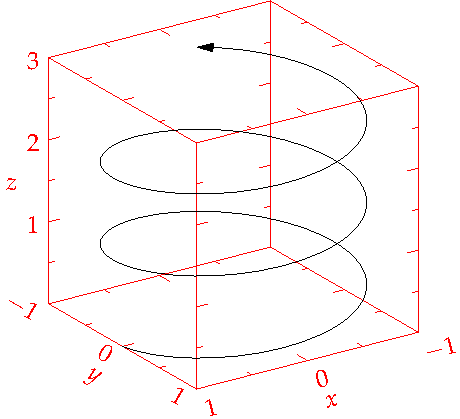
\includegraphics[width=\linewidth]{helix}
  \caption{This is a margin figure.  The helix is defined by
  $x = \cos(2\pi z)$, $y = \sin(2\pi z)$, and $z = [0, 2.7]$.  The figure was
  drawn using Asymptote (\url{http://asymptote.sf.net/}).}
  \label{fig:marginfig}
\end{marginfigure}
\begin{Verbatim}
  \begin{marginfigure}
    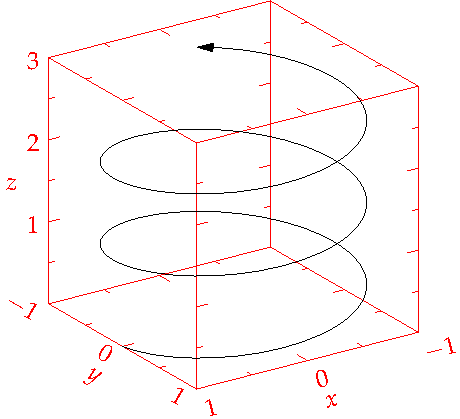
\includegraphics{helix}
    \caption{This is a margin figure.}
  \end{marginfigure}
\end{Verbatim}

The \docenv{marginfigure} and \docenv{margintable} environments accept an
optional parameter \docopt{offset} that adjusts the vertical position of the
figure or table.  See the ``\nameref{sec:sidenotes}'' section above for
examples.  The specifications are:
\begin{docspec}
  \doccmd{begin\{marginfigure\}[\docopt{offset}]}\\
  \qquad\ldots\\
  \doccmd{end\{marginfigure\}}\\
  \mbox{}\\
  \doccmd{begin\{margintable\}[\docopt{offset}]}\\
  \qquad\ldots\\
  \doccmd{end\{margintable\}}\\
\end{docspec}

Figure~\ref{fig:fullfig} is an example of the \Verb|figure*|
environment and figure~\ref{fig:textfig} is an example of the normal
\Verb|figure| environment.

\begin{figure*}[h]
  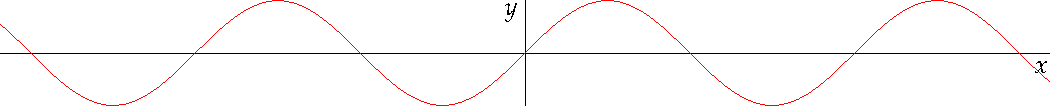
\includegraphics[width=\linewidth]{sine.pdf}%
  \caption{This graph shows $y = \sin x$ from about $x = [-10, 10]$.
  \emph{Notice that this figure takes up the full page
    width.}}%
  \label{fig:fullfig}%
\end{figure*}

\begin{figure}
  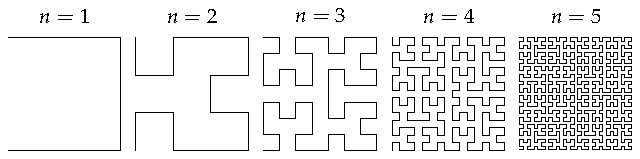
\includegraphics{hilbertcurves.pdf}
  %  \checkparity This is an \pageparity\ page.%
  \caption{Hilbert curves of various degrees $n$.
    \emph{Notice that this figure only takes up the main textblock width.}}
  \label{fig:textfig}
  %\zsavepos{pos:textfig}
  \setfloatalignment{b}
\end{figure}

Table~\ref{tab:normaltab} shows table created with the \docpkg{booktabs}
package.  Notice the lack of vertical rules---they serve only to clutter
the table's data.

\begin{table}[ht]
  \centering
  \fontfamily{ppl}\selectfont
  \begin{tabular}{ll}
    \toprule
    Margin                    & Length                          \\
    \midrule
    Paper width               & \unit[8\nicefrac{1}{2}]{inches} \\
    Paper height              & \unit[11]{inches}               \\
    Textblock width           & \unit[6\nicefrac{1}{2}]{inches} \\
    Textblock/sidenote gutter & \unit[\nicefrac{3}{8}]{inches}  \\
    Sidenote width            & \unit[2]{inches}                \\
    \bottomrule
  \end{tabular}
  \caption{Here are the dimensions of the various margins used in the
    Tufte-handout class.}
  \label{tab:normaltab}
  %\zsavepos{pos:normaltab}
\end{table}

\section{Full-width text blocks}

In addition to the new float types, there is a \docenv{fullwidth}
environment that stretches across the main text block and the sidenotes
area.

\begin{Verbatim}
  \begin{fullwidth}
    Lorem ipsum dolor sit amet...
  \end{fullwidth}
\end{Verbatim}

\begin{fullwidth}
  \small\itshape\lipsum[1]
\end{fullwidth}

\section{Typography}\label{sec:typography}

\subsection{Typefaces}\label{sec:typefaces}
If the Palatino, \textsf{Helvetica}, and \texttt{Bera Mono} typefaces are
installed, this style
will use them automatically.  Otherwise, we'll fall back on the Computer Modern
typefaces.

\subsection{Letterspacing}\label{sec:letterspacing}
This document class includes two new commands and some improvements on
existing commands for letterspacing.

When setting strings of \allcaps{ALL CAPS} or \smallcaps{small caps}, the
letter\-spacing---that is, the spacing between the letters---should be
increased slightly.\cite{Bringhurst2005}  The \Verb|\allcaps| command has
proper letterspacing for
strings of \allcaps{FULL CAPITAL LETTERS}, and the \Verb|\smallcaps| command
has letterspacing for \smallcaps{small capital letters}.  These commands
will also automatically convert the case of the text to upper- or
lowercase, respectively.

The \Verb|\textsc| command has also been redefined to include
letterspacing.	The case of the \Verb|\textsc| argument is left as is,
however.  This allows one to use both uppercase and lowercase letters:
\textsc{The Initial Letters Of The Words In This Sentence Are Capitalized.}

\section{Installation}\label{sec:installation}
To install the Tufte-\LaTeX\ classes, simply drop the
following files into the same directory as your \texttt{.tex}
file:
\begin{quote}
  \ttfamily
  tufte-book.cls\\
  tufte-common.def\\
  tufte-handout.cls\\
  tufte.bst
\end{quote}

% TODO add instructions for installing it globally

\section{More Documentation}\label{sec:more-doc}
For more documentation on the Tufte-\LaTeX{} document classes (including
commands not
mentioned in this handout), please see the sample book.

\section{Support}\label{sec:support}

The website for the Tufte-\LaTeX\ packages is located at
\url{https://github.com/Tufte-LaTeX/tufte-latex}.  On our website, you'll find
links to our \smallcaps{svn} repository, mailing lists, bug tracker, and
documentation.

\bibliography{sample-handout}
\bibliographystyle{plainnat}

\end{document}
